\documentclass[conference,a4paper]{IEEEtran}
\IEEEoverridecommandlockouts

\usepackage[T1]{fontenc}
\usepackage{cite}
\usepackage{amsmath,amssymb,amsfonts}
\usepackage{algorithmic}
\usepackage{graphicx}
\usepackage{textcomp}
\usepackage{xcolor}
\usepackage{microtype}
\usepackage{array}
\usepackage{booktabs}
\usepackage{placeins}
\usepackage{fancyhdr}
\newcolumntype{L}[1]{>{\raggedright\arraybackslash}p{#1}}
\newcolumntype{C}[1]{>{\centering\arraybackslash}p{#1}}
\emergencystretch=2em

\def\BibTeX{{\rm B\kern-.05em{\sc i\kern-.025em b}\kern-.08em
    T\kern-.1667em\lower.7ex\hbox{E}\kern-.125emX}}

% Navigation bookmarks: gives the PDF an outline pane in Acrobat, Edge,
% Okular, VS Code's viewer, etc. hidelinks keeps the printed page identical
% (no coloured or boxed links), so this changes navigation only, not layout.
% hyperref is loaded last, as it must be.
\usepackage[hidelinks,bookmarks=true,bookmarksnumbered=true,
            bookmarksopen=true,bookmarksopenlevel=2,
            pdftitle={How Much Does the Activation Function Matter?
                      A 2000-Run Variance Study of Gated Recurrent Networks
                      for Sentiment Classification},
            pdfsubject={iCONEECT 2026}]{hyperref}

% ── iCONEECT 2026 camera-ready: first-page header and copyright footer ─────
% Both are required on page 1 only. \fancyhf{} clears IEEEtran's own footer,
% so the copyright notice is printed here rather than left to \IEEEpubid;
% \IEEEpubid is still issued after \maketitle so IEEEtran reserves the
% column space and body text cannot collide with the notice.
\fancypagestyle{firstpage}{%
  \fancyhf{}%
  \renewcommand{\headrulewidth}{0pt}%
  \renewcommand{\footrulewidth}{0pt}%
  \fancyhead[L]{\fontsize{9}{10}\selectfont
    \parbox{\textwidth}{2026 1st International Conference on Next-Generation
    Electrical \& Electronics, Computer Systems, and Technologies (iCONEECT).\\
    25--26 September, 2026, Premier University, Chittagong, Bangladesh}}%
  \fancyfoot[L]{\fontsize{9}{10}\selectfont
    979-8-3195-4810-8/26/\$31.00~\copyright2026 IEEE}%
}

\title{How Much Does the Activation Function Matter?\\
A 2{,}000-Run Variance Study of Gated Recurrent\\
Networks for Sentiment Classification}

\author{%
\IEEEauthorblockN{[AUTHOR 1 NAME]}
\IEEEauthorblockA{\textit{[DEPT 1]} \\
\textit{[INSTITUTION 1]}\\{}
[CITY 1], [COUNTRY 1] \\{}
[EMAIL 1]}
\and
\IEEEauthorblockN{[AUTHOR 2 NAME]}
\IEEEauthorblockA{\textit{[DEPT 2]} \\
\textit{[INSTITUTION 2]}\\{}
[CITY 2], [COUNTRY 2] \\{}
[EMAIL 2]}
\and
\IEEEauthorblockN{[AUTHOR 3 NAME]}
\IEEEauthorblockA{\textit{[DEPT 3]} \\
\textit{[INSTITUTION 3]}\\{}
[CITY 3], [COUNTRY 3] \\{}
[EMAIL 3]}
}

\begin{document}
\raggedbottom

% iCONEECT 2026 camera-ready: first-page footer (copyright notice).
% \IEEEpubid must follow \maketitle to take effect on page 1.
\IEEEpubid{\makebox[\columnwidth]{979-8-3195-4810-8/26/\$31.00~\copyright2026
  IEEE\hfill}\hspace{\columnsep}\makebox[\columnwidth]{}}

\maketitle
\thispagestyle{firstpage}
\IEEEpubidadjcol

\begin{abstract}
Activation-function comparisons in gated recurrent networks are
almost always reported from a single training run. It has therefore
never been established whether the differences they report are
larger than the noise of retraining the same model. This paper
settles that question at scale. We train all 100 ordered pairs of ten
activation functions in the dense layers of four gated recurrent
architectures on IMDb, and repeat every one of the 400
configurations under five random seeds, for \textbf{2{,}000 models}
in total with every other setting held fixed. A variance
decomposition over these runs shows that the random seed accounts
for \textbf{58.7\%} of all variation in test accuracy and the
architecture for \textbf{26.7\%}, while the activation pair explains
only \textbf{3.7\%}. The consequence is direct: single-seed
activation rankings do not reproduce. Across the four
architectures the Spearman correlation between the single-seed
ranking of the 100 pairs and their five-seed means is
$-0.174$, $-0.059$, $-0.041$ and $+0.055$, indistinguishable from
zero in every case, and the ten best configurations overlap within
their confidence intervals. What survives is architectural: GRU
outperforms LSTM by 0.79 points ($p<10^{-100}$, Cohen's $d=1.19$),
supplies all fifty highest-scoring configurations, and is the more
reliable choice, with roughly 40\% lower seed-to-seed standard
deviation. One activation effect also survives: smooth
functions reach 73.7\% validation accuracy after one epoch against
61.1\% for the ReLU family. We give the seed budget needed to
resolve each remaining effect, and argue that grid searches of this
kind should report variance as standard.
\end{abstract}

\begin{IEEEkeywords}
Sentiment Analysis, IMDb Dataset, Deep Learning, LSTM, GRU, Activation Functions, Reproducibility, Seed Variance, Experimental Methodology.
\end{IEEEkeywords}

\section{Introduction}

Sentiment analysis is the task of deciding whether a piece of
text is positive or negative. It is one of the most common
problems in natural language processing. The IMDb Large
Movie Review Dataset, with 50{,}000 balanced reviews, is the
standard benchmark for the binary version of the
task~\cite{maas2011}. LSTM and GRU networks are the usual
choice for this problem because their gating mechanisms let
them track context across long sequences~\cite{hochreiter1997,cho2014,chung2014}.

One part of these models gets little attention: the activation
function in the dense layers that sit after the recurrent
layers. The gates inside the recurrent cell are fixed to
sigmoid and tanh, but the dense layers that turn the recurrent
output into a final prediction can use any activation function.
Ahmed et al.~\cite{ahmed2025} tested three classical
combinations in a bidirectional LSTM, reached 88.40\% accuracy,
and asked for follow-up work on modern activation functions and
other architectures.

Answering that call runs into a problem. Every comparison we are
aware of, including all of
\cite{eger2018,farzad2019,essaiAli2022,zhu2022,ahmed2025}, trains
each configuration once. Training is not deterministic. The weight
initialisation, the dropout masks and the order of the training
batches all change the final accuracy, even when the data and every
setting are held identical. If that change is as large as the gaps
between activation functions, then a ranking built from one run per
function is measuring the seed rather than the function. No study
in this area reports how large that change is, so there is no way
to tell which is being measured.

We therefore designed this study around replication. We train all
100 ordered pairs of ten activation functions across four
architectures (LSTM, GRU, and the fully bidirectional version of
each), then repeat every one of those 400 configurations under five
random seeds, holding the data split fixed so that only
initialisation, dropout and batch order vary. The result is
\textbf{2{,}000 trained models}. To our knowledge this is the
largest controlled activation study in gated recurrent networks,
and the first in this setting to report seed variance. Five runs of
every configuration let us measure how much accuracy moves when
only the seed changes, and compare that against the gaps between
activation functions:

\begin{itemize}\itemsep0pt
  \item \textbf{RQ1:} How is accuracy variance divided between
        architecture, activation choice and seed?
  \item \textbf{RQ2:} Does the architecture exceed seed noise?
  \item \textbf{RQ3:} Does the activation pair exceed seed noise?
  \item \textbf{RQ4:} Does a single-seed ranking reproduce?
  \item \textbf{RQ5:} Which activation effects survive?
  \item \textbf{RQ6:} How many seeds would the rest require?
\end{itemize}

\FloatBarrier
\section{Literature Review}

Hochreiter and Schmidhuber~\cite{hochreiter1997} introduced
the LSTM to address the vanishing gradient problem in
recurrent networks, using sigmoid and tanh within the
recurrent cell. Cho et al.~\cite{cho2014} proposed the GRU,
which uses two gates and combines the cell and hidden
states. Chung et al.~\cite{chung2014} compared GRU and LSTM
on sequence-modeling tasks and found GRU competitive with
LSTM. Schuster and Paliwal~\cite{schuster1997} introduced
bidirectional recurrent networks, allowing models to use
both past and future context. These studies established
the recurrent architectures used in our comparison.

The activation function literature developed alongside
these architectural advances. Nair and Hinton~\cite{nair2010}
studied ReLU, which avoids saturation for positive inputs
but has zero gradients for negative inputs. Maas et
al.~\cite{maas2013} and Clevert et al.~\cite{clevert2015}
studied LeakyReLU and ELU, which allow nonzero outputs for
negative inputs. Klambauer et al.~\cite{klambauer2017}
introduced SELU with self-normalising properties under
specific conditions. Later work introduced
GELU~\cite{hendrycks2016}, Swish~\cite{ramachandran2017},
and Mish~\cite{misra2020}, while
surveys~\cite{nwankpa2018,apicella2021} reviewed the growing
range of activation functions. These developments motivate
examining their effects in the dense layers following
gated recurrent networks.

Within sentiment analysis, IMDb~\cite{maas2011} is a widely
used binary classification benchmark. Tang et
al.~\cite{tang2015} studied gated recurrent networks for
document-level sentiment classification, and Socher et
al.~\cite{socher2013} introduced the Stanford Sentiment
Treebank. Several studies have examined activation choice.
Eger et al.~\cite{eger2018} compared 21 activations across
eight NLP tasks and also investigated alternative
activations within LSTM cells. Farzad et
al.~\cite{farzad2019} compared 23 activation functions in
a basic LSTM network on IMDb, Movie Review, and MNIST.
Essai Ali et al.~\cite{essaiAli2022} evaluated 26 state
activation functions in LSTM networks on classification
tasks outside sentiment analysis. Zhu and
Tan~\cite{zhu2022} tested a custom activation in simple RNN,
LSTM, and GRU models on IMDb, comparing it with ReLU,
LeakyReLU, ELU, SELU, and tanh. Ahmed et
al.~\cite{ahmed2025} compared three classical activation
pairings in a bidirectional LSTM, reported 88.40\% accuracy,
and suggested examining modern functions and other
architectures.

Our study brings these comparisons into a shared experimental
design. We evaluate all 100 ordered pairs of ten activation
functions in two dense layers across four architectures.
These use LSTM or GRU cells, a bidirectional first recurrent
layer, and either a unidirectional or bidirectional second
layer. The comparison includes GELU, SiLU, and Mish, with
the data split and training settings held fixed.

Repeated training is also part of earlier work. Eger et
al.~\cite{eger2018} explicitly averaged results over five
random weight initializations in their sentence-classification
experiments. Our main contribution is therefore the analysis
of how variation between training runs compares with the
effects of architecture and dense-layer activation choice
in this setting. We train every configuration with five
seeds and examine whether rankings from one run agree with
rankings based on repeated runs. This allows us to assess
which performance differences are clear and which remain
uncertain.
\FloatBarrier
\section{Methodology}
%------------------------------------------------------------------------------
\subsection{Dataset and Preprocessing}

The IMDb Large Movie Review Dataset~\cite{maas2011} (50,000
reviews, balanced binary labels) was split 80/20 train-test
with \texttt{random\_state=42}, and 10\% of
training data was withheld as a validation set. Reviews were
cleaned by removing HTML tags and non-alphabetic characters,
then lowercased. A vocabulary of the 5,000 most frequent
training-set tokens was used; all sequences were truncated or
zero-padded to 200 tokens.

\subsection{Network Architecture}

All four experiments share the same model structure. The
only thing that changes within each experiment is the choice of
Act$_1$ and Act$_2$ in the two dense layers. The shared architecture
is: an embedding layer
(vocabulary 5,000, dimension 128), a bidirectional recurrent
Layer~1 (64 units per direction), a recurrent Layer~2 (32
units per direction), Dropout(0.4), Dense Layer~1 (64 units)
with Act$_1$, Dense Layer~2 (32 units) with Act$_2$, and a
single output unit trained with \texttt{BCEWithLogitsLoss}.
The four experiments differ only in the recurrent cell type
(LSTM, GRU) and whether Layer 2
is bidirectional (Table~\ref{tab:architectures}).

\begin{table}[htbp]
  \caption{Experimental Architecture Summary}
  \label{tab:architectures}
  \centering
  \footnotesize
  \setlength{\tabcolsep}{4pt}
  \renewcommand{\arraystretch}{1.08}
  \begin{tabular}{cllr}
    \toprule
    Exp. & Layer 1 & Layer 2 & Params \\
    \midrule
    1 & BiLSTM(64) & LSTM(32)    & ${\approx}$764K \\
    2 & BiGRU(64)  & GRU(32)     & ${\approx}$734K \\
    3 & BiLSTM(64) & BiLSTM(32)  & ${\approx}$787K \\
    4 & BiGRU(64)  & BiGRU(32)   & ${\approx}$752K \\
    \bottomrule
  \end{tabular}
\end{table}

\subsection{Activation Functions Under Investigation}

Ten activation functions were evaluated
(Table~\ref{tab:activations}). The classical family is
ReLU~\cite{nair2010}, LeakyReLU~\cite{maas2013},
PReLU~\cite{he2015}, ELU~\cite{clevert2015}, Tanh and
SELU~\cite{klambauer2017}. The modern smooth family is
GELU~\cite{hendrycks2016}, SiLU (Swish)~\cite{ramachandran2017},
Mish~\cite{misra2020} and Hardswish~\cite{howard2019}. The latter
four had not previously been benchmarked in gated recurrent dense
layers for sentiment classification.

\begin{table}[htbp]
  \caption{Activation Functions: Families and Key Properties}
  \label{tab:activations}
  \centering\footnotesize
  \setlength{\tabcolsep}{3pt}
  \renewcommand{\arraystretch}{1.05}
  \resizebox{\columnwidth}{!}{%
  \begin{tabular}{lll}
    \toprule
    Function & Type & Formula / Key Property \\
    \midrule
    ReLU      & Classical & $\max(0,x)$; dead neurons for $x{<}0$ \\
    ELU       & Classical & $\alpha(e^x{-}1)$ for $x{\leq}0$; mean-centering \\
    LeakyReLU & Classical & $0.01x$ for $x{<}0$; low dead-neuron risk \\
    Tanh      & Classical & Bounded; saturates for $|x|\gg1$ \\
    GELU      & Modern & $x\cdot\Phi(x)$; probabilistic gating \\
    SiLU      & Modern & $x\cdot\sigma(x)$; self-gating \\
    Mish      & Modern & $x\cdot\tanh(\text{softplus}(x))$; smooth \\
    SELU      & Modern & Self-normalising; implicit batch norm \\
    PReLU     & Modern & Learnable slope $a$; input-dependent \\
    Hardswish & Modern & Piecewise; dead zone for $x{<}{-3}$ \\
    \bottomrule
  \end{tabular}%
  }
\end{table}

\subsection{Training Configuration and Evaluation}

Every setting in Table~\ref{tab:hyperparams} was held the
same across all runs, so the activation pair is the only
thing that changes between models. The architecture parameters
(vocabulary, embedding, layer sizes, dropout) replicate
Ahmed et al.~\cite{ahmed2025} exactly. The training parameters
(optimizer, learning rate, batch size, scheduler, clipping)
were chosen by us because Ahmed et al. did not report them.
After training, accuracy, precision, recall, and F1-score were
measured on the held-out 10,000-review test set.

\subsection{Replication Protocol}
\label{sec:replication}

Each of the $10\times10\times4 = 400$ configurations was trained
under five seeds, $\{10,20,30,40,50\}$, giving $2{,}000$ models.
The seed is applied immediately before the model and its data
loaders are constructed, setting \texttt{random}, \texttt{numpy},
\texttt{torch} and \texttt{torch.cuda} with
\texttt{cudnn.deterministic=True}, so a given (pair, seed) is
exactly reproducible.

The split is deliberately \emph{not} a function of the seed: it
stays pinned at \texttt{random\_state=42}. The variance we report
is therefore the variance of retraining the same model on the same
data. That is the quantity a single-run comparison assumes to be
negligible. Split variance would only inflate it, so these
estimates are conservative.

Runs were executed five at a time, one worker per seed. Each
worker is a separate process with its own RNG and deterministic
kernel selection, so concurrency cannot perturb a result; we
confirmed this by re-running sampled configurations serially and
recovering identical metrics.

\begin{table}[htbp]
  \caption{Shared Hyperparameter Configuration}
  \label{tab:hyperparams}
  \centering\footnotesize
  \setlength{\tabcolsep}{3pt}
  \renewcommand{\arraystretch}{1.05}
  \resizebox{\columnwidth}{!}{%
  \begin{tabular}{lll}
    \toprule
    Hyperparameter & Value & Source \\
    \midrule
    Vocab / Seq.\ length / Embed. & 5{,}000 / 200 / 128 & \cite{ahmed2025} \\
    RNN Layer 1 / Layer 2 units   & 64 / 32 per direction & \cite{ahmed2025} \\
    Dense Layer 1 / Layer 2 units & 64 / 32 & \cite{ahmed2025} \\
    Dropout rate                  & 0.4 & \cite{ahmed2025} \\
    Batch size / Max epochs       & 64 / 10 & Ours \\
    Early stopping patience       & 3 epochs (val.\ loss) & Ours \\
    Optimiser                     & Adam, $\text{lr}=10^{-3}$ & Ours \\
    LR scheduler                  & ReduceLROnPlateau ($\times$0.5) & Ours \\
    Loss / Gradient clipping      & BCEWithLogitsLoss / $L_2\leq1.0$ & Ours \\
    Weight initialisation         & Kaiming uniform (Linear) & PyTorch default \\
    Data split seed               & 42, fixed for all runs & Ours \\
    Training seeds                & 10, 20, 30, 40, 50 & Ours \\
    \bottomrule
  \end{tabular}%
  }
\end{table}

\subsection{On Reproducing the Baseline of Ahmed et al.}
\label{sec:baseline_repro}

Ahmed et al.~\cite{ahmed2025} describe their architecture in full
and we copy it exactly, but they do not report how they trained
it: optimizer, learning rate, batch size, epochs, early stopping,
seed and data split are all missing. Exact reproduction is
therefore impossible, and we adopt the fully documented settings of
Table~\ref{tab:hyperparams} instead.

Replication sharpens what can be said about their 88.40\%. Our best
configuration averages 87.81\% with a 95\% upper bound of 88.01\%,
and no run among the 2{,}000 reached 88.40\% (maximum 88.39\%), so
the benchmark sits outside the interval of our strongest setting.
Since they report a single run without a seed or standard
deviation, and we measure the per-cell standard deviation of this
model family at 0.38 points, their figure is best read as one draw
of unknown uncertainty. We treat it as a reference point, not a
target.
%------------------------------------------------------------------------------
\FloatBarrier
\section{Results}
\label{sec:results}

\subsection{Where the Variance Comes From}

Test accuracy differs from run to run for three reasons: the
architecture, the activation pair, and the random seed.
Table~\ref{tab:variance} splits the total variance across the
2{,}000 runs between them.

The seed accounts for \textbf{58.7\%}. This is variance between
runs that differ in nothing but the seed, so no choice of
architecture or activation removes it. The architecture accounts
for 26.7\%, almost all of it (26.3\%) from the choice of LSTM or
GRU cell; making the second recurrent layer bidirectional accounts
for 0.19\%. The activation pair accounts for \textbf{3.7\%}.

\begin{table}[htbp]
  \caption{Sources of Variation in Test Accuracy (2{,}000 Runs)}
  \label{tab:variance}
  \centering\footnotesize
  \setlength{\tabcolsep}{4pt}
  \renewcommand{\arraystretch}{1.08}
  \begin{tabular}{@{}lr@{}}
    \toprule
    Source of variation & \% of total variance \\
    \midrule
    Architecture (4 types) & 26.69 \\
    Activation pair (100 pairs) & 3.74 \\
    Architecture--activation interaction & 10.90 \\
    Training seed (within configuration) & 58.67 \\
    \midrule
    \textbf{Total} & \textbf{100.00} \\
    \bottomrule
  \end{tabular}

  \vspace{4pt}
  \parbox{\columnwidth}{\scriptsize
    Each configuration uses one architecture and one activation
    pair. Seed variation is measured across its five training
    runs. The interaction measures how differences between
    activation pairs change across architectures.
  }
\end{table}

The activation effect is about sixteen times smaller than the seed
effect. A study that trains each configuration once measures the
two together and cannot separate them. Section~\ref{sec:rq6} gives
the number of seeds each effect needs.

\subsection{Classification Performance}

Fig.~\ref{fig:architecture_spread} plots the mean accuracy of each
of the 400 configurations, grouped by architecture. Every
architecture mean comes from 500 runs, which gives a 95\%
confidence interval of $\pm$0.03 to $\pm$0.10 points.

The two GRU architectures both average 87.48\% and cannot be told
apart. Both are above the two LSTM architectures, at 86.62\% and
86.75\%. Within each architecture the 100 activation pairs form
one narrow cloud, and the gap between the GRU and LSTM clouds is
wider than any cloud. Changing the cell type moves accuracy more
than changing the activation pair does.

\begin{figure}[htbp]
  \centering
  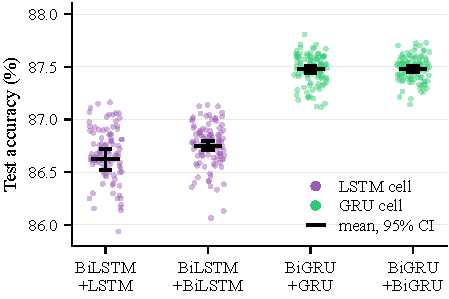
\includegraphics[width=0.92\columnwidth]{assets/architecture_spread.pdf}
  \caption{The 400 replicated cell means, grouped by architecture.
  Each point is one activation pair averaged over five seeds; black
  markers give the architecture mean with its 95\% confidence
  interval. The $y$-axis is truncated at 85.8\%, which clips one
  outlier cell (Hardswish + LeakyReLU in BiLSTM+LSTM, 82.06\%,
  $\sigma=9.27$).}
  \label{fig:architecture_spread}
\end{figure}

Pooling by cell type over 1{,}000 runs each, GRU reaches
$87.48\pm0.02$\% and LSTM $86.69\pm0.05$\%. The gap of
\textbf{0.79} points is large relative to its uncertainty
(Welch $t=26.7$, $p\approx2\times10^{-125}$, Cohen's $d=1.19$).
No configuration's mean reaches the 88.40\% benchmark of Ahmed et
al.~\cite{ahmed2025}; the best cell mean is 87.81\% with a 95\%
upper bound of 88.01\%, and none of the 2{,}000 individual runs
attained 88.40\% (maximum 88.39\%). We therefore treat that figure
as unmatched under our documented training settings rather than as
a target we reached.

\subsection{The Ten Best Configurations}

Table~\ref{tab:top_configs} lists the ten highest-scoring
configurations of the 400, each with its standard deviation and
95\% confidence interval. All ten use a GRU cell, as do the top
fifty.

The ten means lie between 87.68\% and 87.81\%, a spread of
\textbf{0.12} points. Their confidence intervals are wider than
that, up to $\pm$0.50 points. Every interval overlaps every other,
and one range of values is consistent with all ten at once.
\emph{Nothing in the data separates these ten configurations}, so
the order of the rows in Table~\ref{tab:top_configs} is not a
ranking.

\begin{table}[htbp]
  \caption{Ten Highest-Accuracy Configurations of 400, with Seed Variability}
  \label{tab:top_configs}
  \centering\footnotesize
  \renewcommand{\arraystretch}{1.1}
  \resizebox{\columnwidth}{!}{%
  \begin{tabular}{llccc}
    \toprule
    Act$_1$ + Act$_2$ & Experiment & Acc.\% & 95\% CI & F1\% \\
     &  & mean $\pm$ $\sigma$ & $\pm$ & mean \\
    \midrule
    ReLU + LeakyReLU & BiGRU+GRU & 87.81 $\pm$ 0.17 & 0.21 & 87.80 \\
    SiLU + Mish & BiGRU+BiGRU & 87.73 $\pm$ 0.16 & 0.20 & 87.65 \\
    Tanh + LeakyReLU & BiGRU+BiGRU & 87.72 $\pm$ 0.40 & 0.50 & 87.70 \\
    Tanh + GELU & BiGRU+GRU & 87.71 $\pm$ 0.29 & 0.36 & 87.75 \\
    PReLU + ReLU & BiGRU+GRU & 87.71 $\pm$ 0.17 & 0.22 & 87.67 \\
    GELU + GELU & BiGRU+BiGRU & 87.70 $\pm$ 0.18 & 0.22 & 87.58 \\
    SiLU + Hardswish & BiGRU+BiGRU & 87.70 $\pm$ 0.10 & 0.12 & 87.69 \\
    GELU + Hardswish & BiGRU+BiGRU & 87.69 $\pm$ 0.18 & 0.23 & 87.65 \\
    SiLU + GELU & BiGRU+GRU & 87.68 $\pm$ 0.18 & 0.22 & 87.63 \\
    PReLU + GELU & BiGRU+GRU & 87.68 $\pm$ 0.28 & 0.34 & 87.71 \\
    \bottomrule
    \multicolumn{5}{l}{\small All ten are GRU-based. The ten means span 0.12 points, less than} \\
    \multicolumn{5}{l}{\small the widest half-interval ($\pm$0.50); every pair of intervals overlaps.} \\
  \end{tabular}%
  }
\end{table}


\subsection{Reproducibility of the Single-Seed Ranking}

We ranked the 100 activation pairs in each architecture twice:
once by the accuracy of the original single run, and once by the
five-seed mean. Table~\ref{tab:reproducibility} compares the two
rankings.

\begin{table}[htbp]
  \caption{Agreement Between the Single-Seed Ranking and the 5-Seed Means}
  \label{tab:reproducibility}
  \centering\footnotesize
  \setlength{\tabcolsep}{3pt}
  \renewcommand{\arraystretch}{1.1}
  \resizebox{\columnwidth}{!}{%
  \begin{tabular}{lcccc}
    \toprule
    Experiment & $\rho$ & Mean rank $\Delta$ & Top-10 overlap & Mean $|\Delta$acc$|$ \\
    \midrule
    BiLSTM+LSTM & $-0.174$ & 36.9 & 0/10 & 0.53 \\
    BiGRU+GRU & $-0.059$ & 34.5 & 1/10 & 0.34 \\
    BiLSTM+BiLSTM & $-0.041$ & 34.4 & 1/10 & 0.45 \\
    BiGRU+BiGRU & $+0.055$ & 32.1 & 0/10 & 0.36 \\
    \bottomrule
    \multicolumn{5}{l}{\small $\rho$ is the Spearman correlation between the 100 single-seed cell} \\
    \multicolumn{5}{l}{\small accuracies and the corresponding 5-seed means. $\rho\!\approx\!0$ in all four.} \\
  \end{tabular}%
  }
\end{table}


The Spearman correlation between the two rankings is $-0.174$,
$-0.059$, $-0.041$ and $+0.055$ in the four architectures. A
correlation of zero means the first ranking says nothing about the
second, and all four values are close to zero. A pair moves 32 to
37 places out of 100 on average between the two lists. Of the ten
pairs that led each single-seed sweep, at most one is still in the
top ten after replication.

The cause is selection bias. A pair reaches the top of a
single-seed sweep partly because it is good and partly because its
one run was lucky. LeakyReLU + Tanh led the BiGRU+GRU sweep at
88.05\%. Its five runs are 86.70, 87.13, 87.45, 87.46 and 88.20, so
the published figure was its best draw; its mean is
$87.39\pm0.55$, which ranks 77th of 100. The pair that leads on the
mean, ReLU + LeakyReLU, scores $87.81\pm0.17$. The single-seed
winners of the other three architectures fall to ranks 98, 91 and
85. Averaged over the ten leaders of the original sweep, replication
costs 0.48 points.

\subsection{Marginal Effects per Activation}

Averaging each function over all ten of its partners and all five
seeds gives 50 runs per estimate, which removes most of the noise.
A small signal appears at that level: the ten averages within one
architecture span at most 0.67 points, and within BiGRU+GRU only
0.18.

The orderings still do not agree between architectures. Comparing
the four architectures pairwise gives six rank correlations, from
$-0.164$ to $+0.576$, none significant at the 5\% level
($p\geq0.082$). A single-seed reading of this grid suggested that a
function good in one architecture was bad in another, with ELU as
the example: best Act$_1$ in BiGRU+GRU and last in BiLSTM+LSTM.
Replicated, ELU ranks 9th of ten in BiGRU+GRU and 3rd in
BiLSTM+LSTM, so both halves of that claim reverse. The orderings
are unrelated rather than inverted. Per-function averages for all
four architectures are given in the supplementary material.

\subsection{Convergence Speed}

The main sweep records only final accuracy. To measure learning
speed we re-ran the ten homogeneous pairs (X+X) on BiGRU+GRU with
per-epoch logging under five seeds
(Table~\ref{tab:convergence}, Fig.~\ref{fig:convergence_curves}).

\begin{table}[htbp]
  \caption{Epoch-1 Convergence on BiGRU+GRU, Five Seeds}
  \label{tab:convergence}
  \centering\footnotesize
  \renewcommand{\arraystretch}{1.05}
  \resizebox{\columnwidth}{!}{%
  \begin{tabular}{lccc}
    \toprule
    Activation & Val.\ loss (E1) & Val.\ acc.\ (E1)\% & $\sigma$ \\
    \midrule
    Hardswish & 0.523 & \textbf{74.55} & 4.05 \\
    GELU & 0.541 & 74.21 & 3.32 \\
    Mish & 0.544 & 74.03 & 5.97 \\
    SiLU & 0.558 & 72.00 & 3.95 \\
    PReLU & 0.625 & 66.87 & 2.22 \\
    Tanh & 0.651 & 62.76 & 7.52 \\
    LeakyReLU & 0.655 & 62.40 & 4.73 \\
    ELU & 0.644 & 62.20 & 7.29 \\
    ReLU & 0.652 & 61.51 & 7.50 \\
    SELU & 0.674 & 59.24 & 3.73 \\
    \bottomrule
    \multicolumn{4}{l}{\small Smooth family (Mish, GELU, SiLU, Hardswish) averages 73.70\%;} \\
    \multicolumn{4}{l}{\small the ReLU family (ReLU, LeakyReLU, SELU) averages 61.05\%.} \\
  \end{tabular}%
  }
\end{table}


This is the one activation effect in the study that
survives replication. After a single epoch the smooth family
(Mish, GELU, SiLU, Hardswish) averages \textbf{73.70\%}
validation accuracy against \textbf{61.05\%} for the ReLU family
(ReLU, LeakyReLU, SELU). The 12.65-point gap is 2.9 times the
median per-function seed standard deviation of 4.39, and the
ordering is preserved against the single-seed measurement
(Spearman $\rho=0.891$, $p=0.0005$). The advantage is in speed
only: by epoch three all functions reach comparable validation
loss, and the final test accuracies are within noise of each other.

\begin{figure}[htbp]
  \centering
  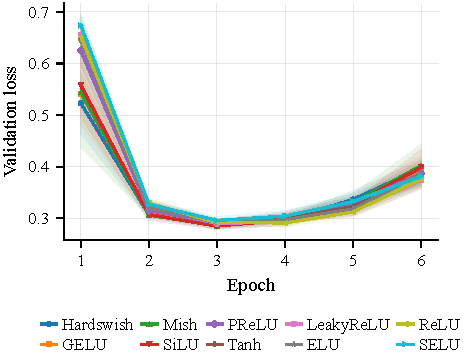
\includegraphics[width=0.92\columnwidth]{assets/convergence_curves.pdf}
  \caption{Per-epoch validation loss on BiGRU+GRU for the ten
  homogeneous pairs. Curves are means over five seeds; shaded
  bands are $\pm1$ standard deviation. The separation visible at
  epoch~1 has closed by epoch~3.}
  \label{fig:convergence_curves}
\end{figure}

\subsection{Reliability and Failure Modes}

Accuracy is not the only axis on which the architectures differ.
The median per-cell standard deviation is 0.30 for the GRU family
against 0.50 for the LSTM family ($p\approx2\times10^{-7}$): GRU is
both more accurate and about 40\% more stable run-to-run.
Instability is also concentrated. Of the eight cells whose standard
deviation exceeds 1.0 point, \emph{all eight} are LSTM-family. The
extreme case, Hardswish + LeakyReLU in BiLSTM+LSTM, averages
82.06\% with $\sigma=9.27$ and a range of 65.50--86.85\%: it trains
normally under four seeds and collapses under the fifth. Apart from
that collapse, no run of the 2{,}000 fell below 60\% accuracy.

Two claims from the single-seed reading do not survive. Per-cell
precision--recall imbalance is one: the widest gap between mean
precision and mean recall over any cell is 6.89 points while
individual runs reach 24.17, so large gaps belong to runs, not to
configurations. A dense-layer ReLU penalty is the other; in
BiLSTM+LSTM, ReLU is the strongest Act$_1$ choice (86.83\% versus
86.60\%, $p=0.006$).

The campaign cost about six GPU-hours on one NVIDIA RTX 5080 at
13.4~s per run. GRU models carry 3.8\% fewer parameters than their
LSTM counterparts (734K versus 764K), making BiGRU+GRU the
cheapest, joint most accurate and most stable of the four.

\FloatBarrier
\section{Discussion}
\label{sec:discussion}

\subsection{RQ1--RQ3: What Actually Moves Accuracy}

We have not found a prior estimate of the variance split for gated
recurrent networks. It sets a limit on what a single-run study can
show: an effect worth 3.7\% of the variance cannot be read off a
design whose noise is worth 58.7\%.

The cell-type effect is large next to the noise, at $d=1.19$, and
four seeds per cell are enough to detect it. It is also the one
conclusion of the original single-seed design that replication
leaves intact: the five-seed architecture means differ from the
single-seed means by at most 0.18 points. Layer-2
bidirectionality is the opposite case. It accounts for 0.19\% of
the variance, and adds 0.13 points in LSTM ($p=0.017$) and 0.00
points in GRU ($p=0.858$). In the GRU case, which is the faster and
more accurate family, the extra parameters add nothing.

The activation pair separates from the noise only when many runs
are averaged. Within BiGRU+GRU the 100 cell means span 0.69 points,
while a single cell has a standard deviation of 0.33 across its
seeds. Averages over ten partners therefore separate; individual
pairs do not. The gap between the LSTM and GRU families, 0.79
points, is larger than the whole 0.69-point span of activation
choices inside GRU.

\subsection{RQ4: Single-Seed Rankings Do Not Reproduce}

In all four architectures the single-seed and five-seed rankings of
the 100 activation pairs are unrelated
(Table~\ref{tab:reproducibility}).

The models themselves are stable. Almost every run lands in a
narrow band, and only one configuration in 400 failed to train
reliably. The problem is the size of the gaps being ranked. Two
pairs adjacent in the ranking differ by about 0.005 points, while a
single pair varies by 0.29 to 0.53 points across its own five
seeds. The noise is roughly eighty times the gap, so one run per
pair sorts seeds rather than functions.

\subsection{RQ5--RQ6: What Survives, and at What Cost}
\label{sec:rq6}

One activation effect survives cleanly: early convergence. Smooth
functions reach 73.70\% validation accuracy after one epoch against
61.05\% for the ReLU family, 2.9 times the seed standard deviation
with the ordering preserved ($\rho=0.891$). Where the budget is
measured in epochs, that is a reason to prefer Mish, GELU, SiLU or
Hardswish. A second effect survives in weaker form: the GRU family
is more stable, and every high-variance cell in the grid is
LSTM-based. Reliability is rarely reported when architectures are
compared; here it points the same way as accuracy. What does not
survive is the identity of the best pair, the transfer or inversion
of rankings across architectures, per-cell precision--recall
behaviour, and any penalty for dense-layer ReLU.

The number of seeds needed to resolve each effect follows from its
size. Taking the median per-cell standard deviation of 0.38 points,
at 80\% power and $\alpha=0.05$, detecting the 0.79-point
architecture effect needs about \textbf{4} seeds per cell, which
is why five were enough here. Separating the top-ranked cell from
the tenth, a gap of 0.12 points, needs about \textbf{157} seeds per
cell. Separating cells adjacent in the top ten needs several
thousand. At the measured 13.4~s per run, the 157-seed case alone
is about 230 GPU-hours for one architecture.

This is the answer to which activation pair is best. It is not that
the winner escaped us: the gaps are small enough that identifying
one would take a budget far beyond what studies in this area spend,
and naming a winner from a single run measures the seed.

\subsection{Limitations}

The study covers one dataset and one task family, so the variance
split should be re-estimated before being assumed elsewhere. The
data split is held fixed by design, so our estimates exclude split
variance and are lower bounds. Five seeds suffice for the
architectural conclusions, but leave per-cell intervals wide
relative to the differences between cells, so individual cell means
should be read with their intervals attached.

\section{Conclusion}

We trained 2{,}000 models, testing 100 activation pairs across
four recurrent architectures with five seeds each. Training
seeds accounted for 58.7\% of the variation in test accuracy,
compared with 26.7\% for architecture and 3.7\% for activation
pairs.

Our main contribution is showing how repeated training changes
the conclusions of an activation comparison. Earlier studies
discussed in this paper reported rankings from single runs.
In our experiments, those rankings showed little agreement
with five-run rankings, moving more than 32 places on average.
This challenges the use of a single run as evidence that one
activation pair is better than another.

Architecture differences were clearer. GRU exceeded LSTM by
0.79 percentage points, supplied all fifty highest-scoring
configurations, and showed about 40\% lower standard deviation
across seeds. Making the second GRU layer bidirectional added
no measurable accuracy benefit.

Activation choice mainly affected early learning. Mish, GELU,
SiLU and Hardswish averaged 73.70\% validation accuracy after
one epoch, compared with 61.05\% for ReLU, LeakyReLU and SELU.
Their early advantage did not produce a clear difference in
final test accuracy.

Under our IMDb settings, architecture choice deserves more
attention than small differences between activation pairs.
More broadly, claims of better performance should be supported
by repeated runs and reported uncertainty. Future work should
test these findings on other datasets, different data splits,
and attention-based models.

{\footnotesize
\begin{thebibliography}{23}
\setlength{\itemsep}{-2.2pt}

% -- Gated Recurrent Architectures --

\bibitem{hochreiter1997}
S. Hochreiter and J. Schmidhuber,
``Long short-term memory,''
\textit{Neural Computation}, vol.~9, no.~8, pp.~1735--1780, Nov. 1997.

\bibitem{cho2014}
K. Cho, B. van Merri\"{e}nboer, C. Gulcehre, D. Bahdanau, F. Bougares,
H. Schwenk, and Y. Bengio,
``Learning phrase representations using RNN encoder-decoder for statistical
machine translation,''
in \textit{Proc. EMNLP}, 2014, pp.~1724--1734.

\bibitem{chung2014}
J. Chung, C. Gulcehre, K. Cho, and Y. Bengio,
``Empirical evaluation of gated recurrent neural networks on sequence
modeling,''
\textit{arXiv preprint arXiv:1412.3555}, 2014.

\bibitem{schuster1997}
M. Schuster and K.~K. Paliwal,
``Bidirectional recurrent neural networks,''
\textit{IEEE Trans. Signal Process.}, vol.~45, no.~11,
pp.~2673--2681, Nov. 1997.

% -- Activation Functions --

\bibitem{nair2010}
V. Nair and G.~E. Hinton,
``Rectified linear units improve restricted Boltzmann machines,''
in \textit{Proc. ICML}, 2010, pp.~807--814.

\bibitem{maas2013}
A.~L. Maas, A.~Y. Hannun, and A.~Y. Ng,
``Rectifier nonlinearities improve neural network acoustic models,''
in \textit{Proc. ICML Workshop on Deep Learning for Audio, Speech and
Language Processing}, 2013.

\bibitem{he2015}
K. He, X. Zhang, S. Ren, and J. Sun,
``Delving deep into rectifiers: Surpassing human-level performance on
ImageNet classification,''
in \textit{Proc. ICCV}, 2015, pp.~1026--1034.

\bibitem{clevert2015}
D. Clevert, T. Unterthiner, and S. Hochreiter,
``Fast and accurate deep network learning by exponential linear units
(ELUs),''
\textit{arXiv preprint arXiv:1511.07289}, 2015.

\bibitem{klambauer2017}
G. Klambauer, T. Unterthiner, A. Mayr, and S. Hochreiter,
``Self-normalizing neural networks,''
in \textit{Proc. NeurIPS}, 2017, pp.~971--980.

\bibitem{hendrycks2016}
D. Hendrycks and K. Gimpel,
``Gaussian error linear units (GELUs),''
\textit{arXiv preprint arXiv:1606.08415}, 2016.

\bibitem{ramachandran2017}
P. Ramachandran, B. Zoph, and Q.~V. Le,
``Searching for activation functions,''
\textit{arXiv preprint arXiv:1710.05941}, 2017.

\bibitem{misra2020}
D. Misra,
``Mish: A self regularized non-monotonic activation function,''
in \textit{Proc. BMVC}, 2020.

\bibitem{howard2019}
A. Howard \textit{et al.},
``Searching for MobileNetV3,''
in \textit{Proc. ICCV}, 2019, pp.~1314--1324.

\bibitem{apicella2021}
A. Apicella, F. Donnarumma, F. Isgr\`{o}, and R. Prevete,
``A survey on modern trainable activation functions,''
\textit{Neural Networks}, vol.~138, pp.~14--32, 2021.

\bibitem{nwankpa2018}
C. Nwankpa, W. Ijomah, A. Gachagan, and S. Marshall,
``Activation functions: Comparison of trends in practice and research for
deep learning,''
\textit{arXiv preprint arXiv:1811.03378}, 2018.

% -- Sentiment Analysis --

\bibitem{maas2011}
A.~L. Maas, R.~E. Daly, P.~T. Pham, D. Huang, A.~Y. Ng, and C. Potts,
``Learning word vectors for sentiment analysis,''
in \textit{Proc. ACL}, 2011, pp.~142--150.

\bibitem{ahmed2025}
S.~A. Ahmed \textit{et al.},
``Comparative analysis of activation functions in LSTM models for sentiment
classification,''
\textit{IJARCCE}, vol.~14, no.~4, Apr. 2025.

\bibitem{zhu2022}
Y. Zhu and R. Tan,
``A novel activation function based recurrent neural networks and their
applications on sentiment classification and log anomaly detection,''
\textit{Frontiers in Neurorobotics}, vol.~16, 2022.

\bibitem{socher2013}
R. Socher, A. Perelygin, J. Wu, J. Chuang, C.~D. Manning, A. Ng,
and C. Potts,
``Recursive deep models for semantic compositionality over a sentiment
treebank,''
in \textit{Proc. EMNLP}, 2013, pp.~1631--1642.

\bibitem{tang2015}
D. Tang, B. Qin, and T. Liu,
``Document modeling with gated recurrent neural network for sentiment
classification,''
in \textit{Proc. EMNLP}, 2015, pp.~1422--1432.

% -- Direct Competitors --

\bibitem{eger2018}
S. Eger, P. Youssef, and I. Gurevych,
``Is it time to swish? Comparing deep learning activation functions across
NLP tasks,''
in \textit{Proc. EMNLP}, 2018, pp.~4423--4433.

\bibitem{farzad2019}
A. Farzad, H. Mashayekhi, and H. Hassanpour,
``A comparative performance analysis of different activation functions in
LSTM networks for classification,''
\textit{Neural Computing and Applications}, vol.~31,
pp.~2507--2521, 2019.

\bibitem{essaiAli2022}
M.~H. Essai~Ali, A.~I. Taloba, M.~F. Farhan, and R.~A. Abozeid,
``Developing novel activation functions based deep learning LSTM for
classification,''
\textit{IEEE Access}, vol.~10, pp.~96578--96591, 2022.

\end{thebibliography}
}
\end{document}
